\documentclass[a4paper,11pt]{article}
\usepackage[utf8]{inputenc}
\usepackage{times}

\usepackage{pgfplots}
\pgfplotsset{width=10cm}

\title{Report for assignment 2}
\author{Ankit Bansal (12EC30003)}

\begin{document}

\maketitle

\paragraph{Hashing}
\begin{enumerate}
 \item \textbf{Overview of the code}

The program is divided into two modes of operations Statistics mode and User input mode. For every type of hashing there are two void functions one is for User input mode(eg.  void chainHash() ) and other is for statistics mode (eg. void schainHash() ).
\begin{description}
  \item[Statistics mode:]
 The mode takes two inputs from the user which are the minimun size of table and the  number of elements which are required to be inserted and using rand() it inserts elements in the hash table. If table size is less as comared to the elements to be inserted than  rehashing will take place according to the condition given in the problem statement. In std out cost of all operations for each type of hashing will be printed.
  \item[User Input mode:]
In User input we can do hashing using all four modes of hashing chain, linear, double and quadratic hashing.User will be asked to ceate  a specific hash table and will ask the user to input the operation (search, insert, delete) which he wants to perform and than asks for a value on which operations is to be done.
\end{description}
 \item \textbf{Description of the functions}
\end{enumerate}

For every type of Hash table there are three basic functions hashInsert, hashDelete, hashSearch. Except Chain Hash there are two more functions hashSize for size of table and hashRehash for Rehashing. 
\begin{description}  
\item[Search:]
Search functions returns the location at which the element is present . If element is not present it returns -1.
\item[Insert:]
Insert function first checks whether the element is already present or not . If element is already present then It prints "Element is already present" . If element is not present it will insert that particular element according to the type of hashing.
\item[Delete:]
Delete function first ensure that element is present or not then if element is present it  deletes that element by deleting the node in chain hashing and by equating its value  = inf (as a flag) in  remaining type of hashing.
\item[Rehash:]
In the program Rehash function is used whenever the size of hash table exceeds 75 percent . Rehash functions creates a new table of size more than twice of initial size and again insert all the elements present in the previous table.
\item[Size:]
Size function returns the number of elements present in the Hash Table.
\item[Comparision of collision in different  Hash tables: ]
The graph is created for size of hashtable equals to next prime of 200 ( 211 ) and number of elements to be inserted  varying from 20 to 400 (Load factor 0.1 to 2). In the graph below we can clearly observe that for low load factor all three scheme have more or less same collisions , for large values of load factor Double hashing is the best scheme for hashing. Load factor 2 means initial size of table is 211 and number of elements to be inserted is 422. In this case rehashing will take place leading to a large number of collisions.
\end{description}


% Preamble: \pgfplotsset{width=7cm,compat=1.11}
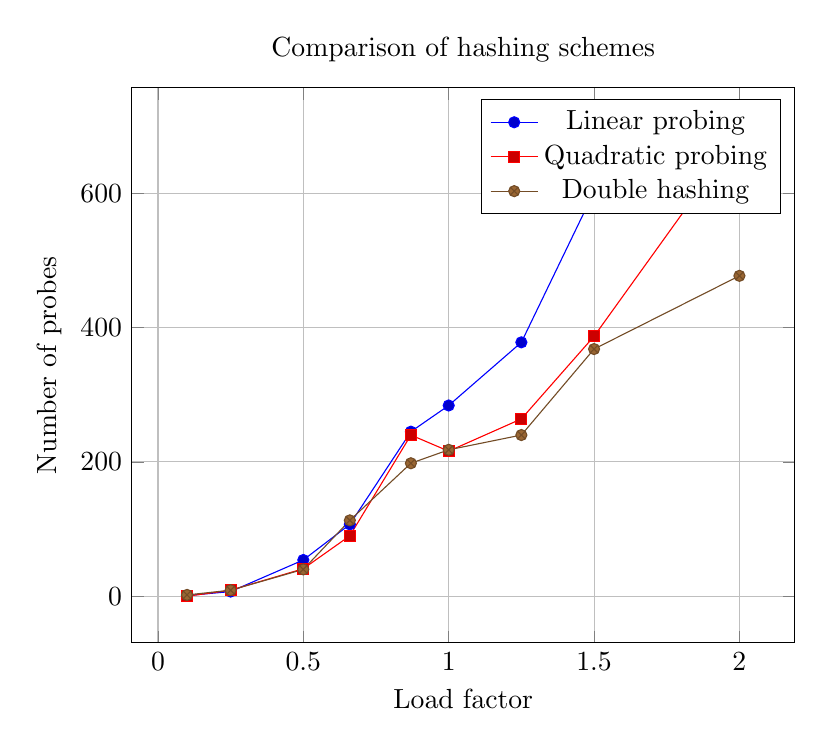
\begin{tikzpicture}
\begin{axis}[
      title=Comparison of hashing schemes,
      xlabel={Load factor},
      ylabel={Number of probes},
      grid=major,
      legend entries={Linear probing,Quadratic probing,Double hashing},
]
\addplot coordinates {
(0.1,1)
(0.25,7)
(0.5,54)
(0.66,107)
(0.87,245)
(1,284)
(1.25,378)
(1.5,602)
(2,605)
};
\addplot coordinates {
(0.1,0)
(0.25,9)
(0.5,41)
(0.66,90)
(0.87,240)
(1,216)
(1.25,264)
(1.5,387)
(2,688)
};
\addplot coordinates {
(0.1,2)
(0.25,9)
(0.5,40)
(0.66,113)
(0.87,198)
(1,218)
(1.25,240)
(1.5,368)
(2,477)
};
\end{axis}
\end{tikzpicture}


\end{document}
